\section{Related work}

The biomass indexes has been widely explored by several researches. Most of them show how useful is use satellite imagery with different resolutions. In general, this researches have as start point a fieldwork where is calculated the biomass nominal value to different samples using traditional laboratory techniques. Subsequently, this results are used and the different bands given by the satellite imagery to infer a model using some regression technique to finally extrapolate to the study area.

As an example, \cite{klemas2013remotesensing} uses this methodology to detect changes in biomass levels at different coast zones at United States using LIDAR imagery and lineal regression. Similarly, \cite{baccini2008afirst} use MODIS imagery and decision trees (in addition to traditional regression techniques) to estimate AGB (Above-Ground Biomass) index at an wide tropical African area. Comparable to this study, \cite{mitchard2009usingsatellite} use radar imagery to predict AGB at four reserve and African national parks classifying different types of earth crust. \cite{muukkonen2007biomass} also use of MODIS imagery in conjunction with ASTER imagery to estimate biomass pursuing an carbon sequestration inventory. An important contribution of this paper is the shared methodology used through the project as is showed the figure~\ref{fig:Mukkonnen01}. \cite{powell2010quantification} introduce the use of new regression techniques (reduced major axis regression, gradient nearest neighbor imputation y ramdom forest regression trees) to generate biomass models this time using Landsat imagery. In \cite{hall2006modeling} is introduced bioSTRUCT, a method to generate correlations between continued values measured by the satellite imagery bands and the AGB measured previously using laboratory techniques. The paper shows the methology as a study case at Alberta (Canada) and open source Landsat imagery ETM+. As a result are obtained regression formulas from the limited number of samples than can be extrapolated to the full study area.

\begin{figure}
  \centering
  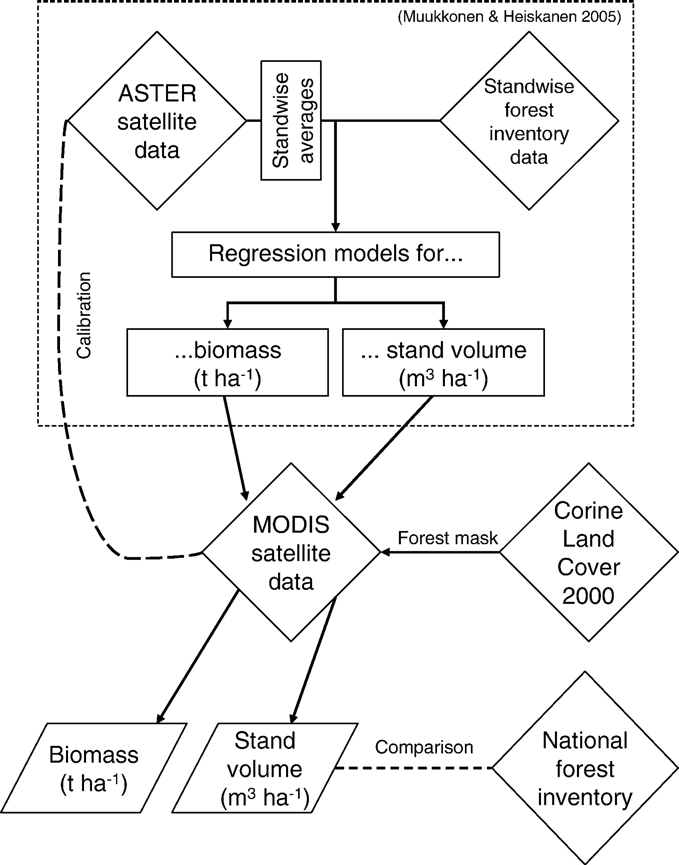
\includegraphics[width = 8cm]{Mukkonnen01.png}
  \caption{Methodology proposed by \cite{muukkonen2007biomass}}
  \label{fig:Mukkonnen01}
\end{figure}